O gerenciamento de riscos em um projeto tem como objetivo orientar a equipe do sobre os riscos presentes, como serão controlados e monitorados, além de aumentar a probabilidade e  impacto de eventos positivos e reduzir a probabilidade e impacto dos eventos negativos.

O processo consiste na realização de um plano de gerenciamento que descreva a análise e execução dos processos de riscos, iniciando-se pela identificação dos mesmos, suas análises quantitativas e qualitativas, plano de respostas e por fim a solução de como eles serão monitorados e controlados durante o ciclo de vida do projeto.

\section{Processo de Gerenciamento de Riscos} % (fold)
\label{sec:processo_de_gerenciamento_de_riscos}
	
	O processo de gerenciamento de riscos nesse projeto, ocorrerá nas seguintes etapas:
	\begin{itemize}
		\item Identificar os riscos e determinar quais deles podem afetar o projeto, documentando suas características.
		\item Realizar a análise qualitativa dos riscos.
		\item Avaliar a exposição ao risco para priorizar os que serão objeto de análise ou ação adicional. 
		\item Realizar a análise quantitativa dos riscos.
		\item Efetuar a análise numérica do efeito dos riscos identificados nos objetivos gerais do projeto.
		\item Planejar as respostas aos riscos, desenvolvendo opções e ações para aumentar as oportunidades e reduzir ameaças aos objetivos do projeto.
		\item Controlar os riscos e monitora-los durante o ciclo de vida do projeto.

	\end{itemize}

% section processo_de_gerenciamento_de_riscos (end)
\section{Responsabilidade dos Riscos da Equipe do Projeto} % (fold)
\label{sec:responsabilidade_dos_riscos_da_equipe_do_projeto}

Os processos de gerenciamento de riscos serão realizados pelo Scrum master de projeto, durante o período, no entanto todos os membros da equipe de desenvolvimento do R2-I2 serão consultados nesse processo para o levantamento de riscos dos sistemas e subsistemas pelos quais estão responsáveis, assim como as formas de controle dos mesmos.

\section{Probabilidade e Impacto de Riscos} % (fold)
 \label{sec:probabilidade_e_impacto_de_riscos}
 
 Diferentes riscos possuem diferentes probabilidades de ocorrência e diferentes impactos no projeto. Tendo isso em vista, foram feitas uma matriz de risco e probabilidade e uma matriz de impacto para auxiliar da qualidade e credibilidade da análise dos riscos assim como na decisão de respostas e plano de controle.

 \subsection{Matriz de Risco e Probabilidade} % (fold)
 \label{sub:matriz_de_risco_e_probabilidade}

 A tabela \ref{tab:probabilidade} mostra a matriz de probabilidade dos riscos com uma pontuação para a análise qualitativa.

 \begin{table}[H]
	\centering
	\caption{Matriz de probabilidade de riscos do R2-PI2.}
	\label{my-label}
	\begin{tabular}{|c|c|}
		\hline
		\rowcolor[HTML]{C0C0C0} 
		\textit{\textbf{Probabilidade}} & \textit{\textbf{\% de certeza}} \\ \hline
		1- Muito baixa                  & 0 a 20\%                        \\ \hline
		2- Baixa                        & 20 a 40\%                       \\ \hline
		3- Média                        & 40 a 60\%                       \\ \hline
		4- Alta                         & 60 a 80\%                       \\ \hline
		5- Muito alta                   & \textgreater80\%                \\ \hline
	\end{tabular}
\end{table}
 
 % subsection matriz_de_risco_e_probabilidade (end)
 \subsection{Matriz de Impacto dos Riscos} % (fold)
 \label{sub:matriz_de_impacto_dos_riscos}
 
 Para chegar em uma nota final de impacto para o risco, foram considerados 4 aspectos principais: Custo, Tempo, Escopo e Qualidade.

 \begin{table}[H]
\centering
\caption{Matriz de impacto de riscos.}
\label{tab:matriz_impacto}
\begin{tabular}{|c|c|c|c|c|c|}
\hline
\multirow{2}{*}{\textit{\textbf{Custo}}}  & \textit{\textbf{\begin{tabular}[c]{@{}c@{}}Muito baixo\\ (nota 1)\end{tabular}}}                                & \textit{\textbf{\begin{tabular}[c]{@{}c@{}}Baixo\\ (nota 2)\end{tabular}}}                & \textit{\textbf{\begin{tabular}[c]{@{}c@{}}Médio\\ (nota 3)\end{tabular}}}                           & \textit{\textbf{\begin{tabular}[c]{@{}c@{}}Alto\\ (nota 4)\end{tabular}}}                                       & \textit{\textbf{\begin{tabular}[c]{@{}c@{}}Muito alto\\ (nota 5)\end{tabular}}}                  \\ \cline{2-6} 
                                          & \begin{tabular}[c]{@{}c@{}}Até 2\% no \\ orçamento\end{tabular}                                                 & \begin{tabular}[c]{@{}c@{}}De 2 a 5\% \\ no orçamento\end{tabular}                        & \begin{tabular}[c]{@{}c@{}}De 5 a 8\% \\ no orçamento\end{tabular}                                   & \begin{tabular}[c]{@{}c@{}}De 8 a 10\% \\ no orçamento\end{tabular}                                             & \begin{tabular}[c]{@{}c@{}}Acima de 10\% \\ no orçamento\end{tabular}                            \\ \hline
\multirow{2}{*}{\textit{\textbf{Tempo}}}  & \multirow{2}{*}{\begin{tabular}[c]{@{}c@{}}Até 2\% no \\ prazo total\end{tabular}}                              & \multirow{2}{*}{\begin{tabular}[c]{@{}c@{}}De 2 a 5\% \\ no prazo\end{tabular}}           & \multirow{2}{*}{\begin{tabular}[c]{@{}c@{}}De 5 a 8\% \\ no prazo\end{tabular}}                      & \multirow{2}{*}{\begin{tabular}[c]{@{}c@{}}De 8 a 10\%\\  no prazo\end{tabular}}                                & \multirow{2}{*}{\begin{tabular}[c]{@{}c@{}}Acima de 10\%\\  no prazo\end{tabular}}               \\
                                          &                                                                                                                 &                                                                                           &                                                                                                      &                                                                                                                 &                                                                                                  \\ \hline
\multirow{2}{*}{\textit{\textbf{Escopo}}} & \multirow{2}{*}{\begin{tabular}[c]{@{}c@{}}Impacto \\ insignificante na\\ qualidade do \\ projeto\end{tabular}} & \multirow{2}{*}{\begin{tabular}[c]{@{}c@{}}Mudança \\ impactará no\\  custo\end{tabular}} & \multirow{2}{*}{\begin{tabular}[c]{@{}c@{}}Mudança \\ impactará no \\ custo e no tempo\end{tabular}} & \multirow{2}{*}{\begin{tabular}[c]{@{}c@{}}Mudança \\ impactará no \\ custo, tempo \\ e qualidade\end{tabular}} & \multirow{2}{*}{\begin{tabular}[c]{@{}c@{}}Produto final \\ do projeto é \\ inútil\end{tabular}} \\
                                          &                                                                                                                 &                                                                                           &                                                                                                      &                                                                                                                 &                                                                                                  \\ 
                                          &                                                                                                                 &                                                                                           &                                                                                                      &                                                                                                                 &      \\ 
                                          &                                                                                                                 &                                                                                           &                                                                                                      &                                                                                                                 &      \\ \hline
\end{tabular}
\end{table}
 % subsection matriz_de_impacto_dos_riscos (end)

 % section probabilidade_e_impacto_de_riscos (end) 
 \section{Planejamento de Resposta aos Riscos} % (fold)
 \label{sec:planejamento_de_resposta_aos_riscos}
 	
 	A partir das outras matrizes apresentadas anteriormente, é criada a matriz de probabilidade e impacto. As notas de impacto e probabilidade foram multiplicadas para chegar a uma nota final de risco.

 	\begin{figure}[H]
		\centering
		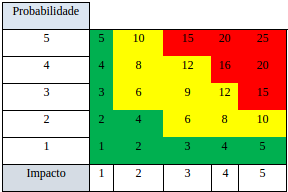
\includegraphics[scale=0.8]{figuras/matriz_probab.png}
		\caption{Matriz de probabilidade e impacto.}
		\label{img:modeloH}
	\end{figure}

	A cor verde na tabela representa risco mínimo. A cor amarela representa risco médio e a cor vermelha representa risco alto. A estratégia a ser adotada para cada escala de risco identificada está apresentada na tabela \ref{tab:legprob}. 

	\begin{table}[H]
		\centering
		\caption{Legenda matriz de probabilidade}
		\label{tab:legprob}
		\begin{tabular}{|c|c|c|c|}
			\hline
			\textit{\textbf{Zona}}                   & \textit{\textbf{Prioridade}} & \textit{\textbf{Pontuação}} & \textit{\textbf{Estratégia}}                                                      \\ \hline
			{\color[HTML]{009901} \textbf{Verde}}    & Baixa                        & de 0 a 4                    & Aceitação                                                                         \\ \hline
			{\color[HTML]{FFCB2F} \textbf{Amarelo}}  & Média                        & de 5 a 14                   & \begin{tabular}[c]{@{}c@{}}Aceitação ou \\ mitigação\end{tabular}                 \\ \hline
			{\color[HTML]{FE0000} \textbf{Vermelho}} & Alta                         & de 16 a 25                  & \begin{tabular}[c]{@{}c@{}}Eliminação, mitigação \\ ou transferência\end{tabular} \\ \hline
		\end{tabular}
	\end{table}
 % section planejamento_de_resposta_aos_riscos (end)


% section responsabilidade_dos_riscos_da_equipe_do_projeto (end)